\tikzset{every picture/.style={line width=0.75pt}} %set default line width to 0.75pt        
\begin{figure}[H]
    \begin{center}
        \caption{Legenda diagrama pneu}
        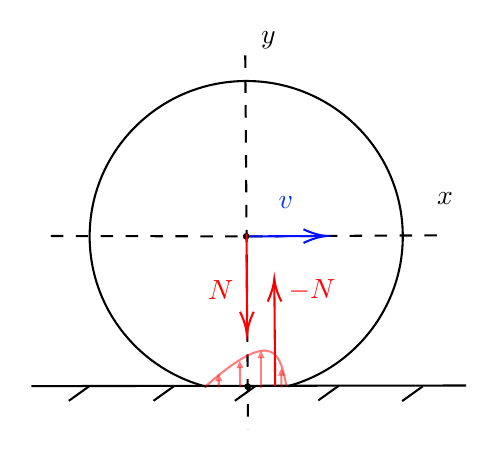
\begin{tikzpicture}[x=0.75pt,y=0.75pt,yscale=-1,xscale=1]
            %uncomment if require: \path (0,189); %set diagram left start at 0, and has height of 189

            %Straight Lines [id:da7518330174479086] 
            \draw  [dash pattern={on 4.5pt off 4.5pt}]  (6.67,90) -- (100.79,90.19) -- (193.33,89.67) ;
            %Straight Lines [id:da5592434503400421] 
            \draw	 (-2.68,162.32) -- (206.73,162.03) ;
            %Shape: Arc [id:dp1726281412706019] 
            \draw  [draw opacity=0][fill={rgb, 255:red, 8; green, 7; blue, 7 }  ,fill opacity=0 ] (81.65,162.63) .. controls (49.67,154.34) and
            (25.87,125.7) .. (25.36,91.3) .. controls (24.76,49.95) and (58.03,15.94) .. (99.69,15.33) .. controls (141.35,14.72) and (175.61,47.74) ..
            (176.22,89.08) .. controls (176.73,124) and (153.08,153.68) .. (120.62,162.44) -- (100.79,90.19) -- cycle ; \draw   (81.65,162.63) .. controls
            (49.67,154.34) and (25.87,125.7) .. (25.36,91.3) .. controls (24.76,49.95) and (58.03,15.94) .. (99.69,15.33) .. controls (141.35,14.72) and
            (175.61,47.74) .. (176.22,89.08) .. controls (176.73,124) and (153.08,153.68) .. (120.62,162.44) ;
            %Straight Lines [id:da003920177628984778] 
            \draw [color={rgb, 255:red, 4; green, 18; blue, 249 }  ,draw opacity=1 ]   (100.79,90.19) -- (137.33,90.01) ;
            \draw [shift={(139.33,90)}, rotate = 539.72] [color={rgb, 255:red, 4; green, 18; blue, 249 }  ,draw opacity=1 ][line width=0.75]
            (10.93,-3.29) .. controls (6.95,-1.4) and (3.31,-0.3) .. (0,0) .. controls (3.31,0.3) and (6.95,1.4) .. (10.93,3.29)   ;
            %Straight Lines [id:da6241641943206588] 
            \draw [color={rgb, 255:red, 0; green, 0; blue, 0 }  ,draw opacity=1 ]	(25.2,162.33) -- (15.33,169.4) ;
            %Straight Lines [id:da6421337551968986] 
            \draw [color={rgb, 255:red, 0; green, 0; blue, 0 }  ,draw opacity=1 ]	(66,162.33) -- (56.13,169.4) ;
            %Straight Lines [id:da25242184369144227] 
            \draw [color={rgb, 255:red, 0; green, 0; blue, 0 }  ,draw opacity=1 ]	(105.2,162.33) -- (95.33,169.4) ;
            %Straight Lines [id:da7965874493492349] 
            \draw [color={rgb, 255:red, 0; green, 0; blue, 0 }  ,draw opacity=1 ]	(145.4,162.13) -- (135.53,169.2) ;
            %Straight Lines [id:da2366122350933053] 
            \draw [color={rgb, 255:red, 0; green, 0; blue, 0 }  ,draw opacity=1 ]	(185.8,162.47) -- (175.93,169.53) ;
            %Straight Lines [id:da201352955590123] 
            \draw  [dash pattern={on 4.5pt off 4.5pt}]  (100.33,3) -- (101.67,183) ;
            %Straight Lines [id:da12037912623915337] 
            \draw	 (-4,15.67) ;
            %Shape: Circle [id:dp21540655765824446] 
            \draw  [color={rgb, 255:red, 0; green, 0; blue, 0 }  ,draw opacity=1 ][fill={rgb, 255:red, 0; green, 0; blue, 0 }  ,fill opacity=1 ]
            (100.45,162.53) .. controls (100.45,161.94) and (100.94,161.45) .. (101.53,161.45) .. controls (102.13,161.45) and (102.62,161.94) .. (102.62,162.53)
            .. controls (102.62,163.13) and (102.13,163.62) .. (101.53,163.62) .. controls (100.94,163.62) and (100.45,163.13) .. (100.45,162.53) -- cycle ;
            %Shape: Circle [id:dp5323977356859111] 
            \draw  [color={rgb, 255:red, 0; green, 0; blue, 0 }  ,draw opacity=1 ][fill={rgb, 255:red, 0; green, 0; blue, 0 }  ,fill opacity=1 ]
            (99.73,89.99) .. controls (99.84,89.4) and (100.4,89.01) .. (100.99,89.13) .. controls (101.58,89.24) and (101.97,89.8) .. (101.85,90.39) .. controls
            (101.74,90.98) and (101.17,91.37) .. (100.59,91.25) .. controls (100,91.14) and (99.61,90.58) .. (99.73,89.99) -- cycle ;
            %Straight Lines [id:da8962219135738276] 
            \draw [color={rgb, 255:red, 255; green, 0; blue, 0 }  ,draw opacity=1 ]   (100.99,89.13) -- (101.13,135.43) ;
            \draw [shift={(101.13,137.43)}, rotate = 269.83] [color={rgb, 255:red, 255; green, 0; blue, 0 }  ,draw opacity=1 ][line width=0.75]
            (10.93,-3.29) .. controls (6.95,-1.4) and (3.31,-0.3) .. (0,0) .. controls (3.31,0.3) and (6.95,1.4) .. (10.93,3.29)	;
            %Straight Lines [id:da7902625791767064] 
            \draw [color={rgb, 255:red, 246; green, 0; blue, 0 }  ,draw opacity=1 ][fill={rgb, 255:red, 254; green, 0; blue, 0 }  ,fill opacity=1
            ]   (114.73,162.23) -- (114.35,112.63) ;
            \draw [shift={(114.33,110.63)}, rotate = 449.56] [color={rgb, 255:red, 246; green, 0; blue, 0 }  ,draw opacity=1 ][line width=0.75]
            (10.93,-3.29) .. controls (6.95,-1.4) and (3.31,-0.3) .. (0,0) .. controls (3.31,0.3) and (6.95,1.4) .. (10.93,3.29)	;
            %Curve Lines [id:da9381909177646195] 
            \draw [color={rgb, 255:red, 255; green, 0; blue, 0 }  ,draw opacity=0.51 ]   (81.25,162.43) .. controls (115.59,132.01) and
            (117.14,148.45) .. (120.22,162.24) ;
            %Straight Lines [id:da46399317653073635] 
            \draw [color={rgb, 255:red, 255; green, 0; blue, 0 }  ,draw opacity=0.51 ]   (87.58,162.88) -- (87.55,159.32) ;
            \draw [shift={(87.53,156.32)}, rotate = 449.5] [fill={rgb, 255:red, 255; green, 0; blue, 0 }  ,fill opacity=0.51 ][line width=0.08]
            [draw opacity=0] (3.57,-1.72) -- (0,0) -- (3.57,1.72) -- cycle	  ;
            %Straight Lines [id:da977275191245905] 
            \draw [color={rgb, 255:red, 255; green, 0; blue, 0 }  ,draw opacity=0.51 ]   (97.93,162.92) -- (97.77,153.12) ;
            \draw [shift={(97.73,150.12)}, rotate = 449.1] [fill={rgb, 255:red, 255; green, 0; blue, 0 }  ,fill opacity=0.51 ][line width=0.08]
            [draw opacity=0] (3.57,-1.72) -- (0,0) -- (3.57,1.72) -- cycle	  ;
            %Straight Lines [id:da7569878460768078] 
            \draw [color={rgb, 255:red, 255; green, 0; blue, 0 }  ,draw opacity=0.51 ]   (107.93,163.12) -- (107.93,148.32) ;
            \draw [shift={(107.93,145.32)}, rotate = 450] [fill={rgb, 255:red, 255; green, 0; blue, 0 }  ,fill opacity=0.51 ][line width=0.08]
            [draw opacity=0] (3.57,-1.72) -- (0,0) -- (3.57,1.72) -- cycle	  ;
            %Straight Lines [id:da6646192752580227] 
            \draw [color={rgb, 255:red, 255; green, 0; blue, 0 }  ,draw opacity=0.51 ]   (117.78,162.93) -- (117.74,156.72) ;
            \draw [shift={(117.73,153.72)}, rotate = 449.64] [fill={rgb, 255:red, 255; green, 0; blue, 0 }	,fill opacity=0.51 ][line width=0.08]
            [draw opacity=0] (3.57,-1.72) -- (0,0) -- (3.57,1.72) -- cycle    ;

            % Text Node
            \draw (114.93,69.33) node [anchor=north west][inner sep=0.75pt]  [color={rgb, 255:red, 3; green, 49; blue, 254 }  ,opacity=1 ]
            {$v$};
            % Text Node
            \draw (80.93,109.93) node [anchor=north west][inner sep=0.75pt]  [color={rgb, 255:red, 249; green, 0; blue, 0 }  ,opacity=1 ]  {$N$};
            % Text Node
            \draw (119.73,109.53) node [anchor=north west][inner sep=0.75pt]  [color={rgb, 255:red, 247; green, 4; blue, 4 }  ,opacity=1 ]
            {$-N$};
            % Text Node
            \draw (191.33,67.53) node [anchor=north west][inner sep=0.75pt]    {$x$};
            % Text Node
            \draw (106.53,-9.87) node [anchor=north west][inner sep=0.75pt]    {$y$};

        \end{tikzpicture}
    \end{center}
    \caption*{\footnotesize Fonte: Elaborado pelo autor.}
    \label{fig:diagramaPeneu}
\end{figure}
